%===================================================================================================
\subsection{Partnership Numbers}\label{model.par.pnum}
This section summarizes the numbers of partnerships modelled among activity groups.
Similar to group sizes, I draw on the
analysis of FSW data in \sref{model.par.fsw} and
bias adjustment for wider population in \sref{model.par.wp}.
However, first in \sref{model.par.pnum.adj},
I critically review the interpretation of reported partner numbers
with regards to partnership duration, and develop a related adjustment.
%---------------------------------------------------------------------------------------------------
\subsubsection{Adjusting for Partnership Duration}\label{model.par.pnum.adj}
Sexual partnerships are usually quantified using cross-sectional surveys.
In this case, respondents are typically asked to report the numbers of unique partners ``$x$''
during a standardized recall period $\omega$
--- \eg \shortquote{How many different people have you had sex with during the past year?}
Such data can then be used to define
a rate of partnership change $Q$ and/or a number of concurrrent partnerships $K$,
depending on the modelled force of infection equation (see Chapter~\ref{foi}).
\par
If partnership duration is long and the recall period is short
--- including $\omega \approx 0$ for
\shortquote{Are you currently in a long-term sexual partnership?} ---
the reported partnerships mostly reflect \emph{ongoing} partnerships,
and thus $x \approx K$.
If partnership duration is short and the recall period is long,
--- including $\delta \approx 0$ for
\shortquote{How many one-off sexual partners have you had during the past year?} ---
the reported partnerships mostly reflect \emph{complete} partnerships,
and thus $x/\omega \approx Q$.
However, if partnership duration and recall period are similar in length,
the reported partnerships reflect a mixture of tail-ends, complete, and ongoing partnerships,
and thus $x$ overestimates $K$, but $x/\omega$ also overestimates $Q$.
In summary:
\begin{itemize}
  \item $\omega \ll \delta$: mostly ongoing partnerships;
  $x \approx K$ (concurrrent)
  \item $\omega \gg \delta$: mostly complete partnerships;
  $x/\omega \approx Q$ (change rate)
  \item $\omega\,\approx\,\delta$: some tail-ends, some complete, some ongoing;
  $x > K$, $x/\omega > Q$ (neither)
\end{itemize}
\par
I developed an approach to estimate $Q$ and $K$ from $x$,
for a known recall period $\omega$ and partnership duration $\delta$.
The average durations of each type of partnership are estimated in \sref{model.par.pdur}.
The approach draws on a similar assumption as in \sref{model.par.turn.act}:
that survey timing is effectively random with respect to partnership duration.
Then, if either end of the recall period would capture an ongoing partnership,
the intersection point would be, on average, at the partnership mid-point.
Thus, the recall period is effectively extended
by half the partnership duration $\delta/2$ on each end, and $\delta$ overall,
as illustrated in Figure~\ref{fig:diag.recall}.
As such, we can define $Q$ and $K$ as:
\begin{alignat}{1}
  Q &= \frac{x}{\omega+\delta} \label{eq:x2Q}\\
  K &= \frac{x\delta}{\omega+\delta} = Q\delta \label{eq:x2K}
\end{alignat}
\begin{figure}
  \centering
  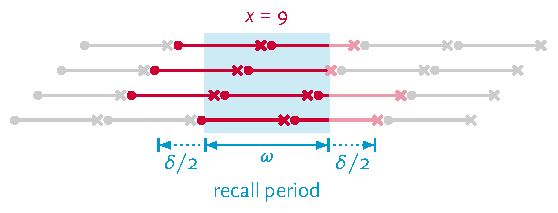
\includegraphics[scale=1]{diag.recall}
  \caption{Illustration of conceptual framework for quantifying partnerships
    from the number reported during a given recall period}
  \label{fig:diag.recall}
  \floatfoot{
    Circle: partnership start; line: ongoing partnership; cross: partnership end;
    $\omega$/red: recall period;
    $\delta$: partnership duration;
    $x$: number of reported partnerships for $\omega$.}
\end{figure}
\par
As an example, Figure~\ref{fig:diag.recall} illustrates
a recall period of $\omega = 1$ year,
for which $x = 9$ partnerships are reported,
having durations of $\delta = 9$ months.
Thus, we can compute $Q = 9/(1+0.75) = 5.14$ and $K = 5.14(0.75) = 3.86$,
which is a slight underestimate of the true values $Q = 5.33, K = 4$,
due to the randomness in the exact ``location'' of the recall period.
%---------------------------------------------------------------------------------------------------
\subsubsection{Sex Work Partnerships}\label{model.par.pnum.sw}
%---------------------------------------------------------------------------------------------------
\paragraph{Female Sex Workers}
Table~\ref{tab:fsw.ratios} summarizes
the numbers of new and regular clients \emph{per month} reported by Swati FSW,
stratified by higher \vs lower risk per the analysis in \sref{model.par.fsw.fac}.
These data thus would provide $x$ for $\omega = 1$ month.
However, based on the survey questions,%
\footnote{The survey questions were: \shortquote{In the last 30 days,
  how many (new/regular) clients have you had sex with?}, or similar.}
it's not clear whether these reported partner numbers
represent the numbers of unique men or unique client visits.
\par
I assumed that all \emph{new} clients were one-off visits;
thus the reported partner numbers effectively represented
$1/12$th of the total numbers of yearly partnerships $Q_{p_{3}}$.
As such, I sampled the yearly rate of new sex work partnerships among lower risk FSW
from a gamma distribution with mean (95\%~CI) as 4.1~(2.5,~6.0) $\times$ 12,
and the \emph{relative} rate among higher risk FSW from 2.0~(1.6,~2.5).
Since each partnership is assumed to include only one sex act,
the partnership duration $\delta_{p_{3}}$, frequency of sex $F_{p_{3}}$,
and number of concurrent partnerships $K_{p_{3}}$ are ill-defined,
but can be defined for convenience as
$\delta_{p_{3}} = 1/12$ (years), $F_{p_{3}} = 12$ (per year),
and $K_{p_{3}} = Q_{p_{3}} / 12$.
\par
For \emph{regular} sex work partnerships, uncertainties remain regarding
partnership duration $\delta_{p_{4}}$ (see \sref{model.par.pdur}),
frequency of sex per month $F_{p_{4}}/12$, and
survey responses $x$ reflecting unique clients or total client visits per month.
If $x$ reflects the numbers of unique clients, then
$Q_{p_{4}s_{1}i_{34}}$ can be defined via \eqref{eq:x2Q} using $x$ directly;
whereas if $x$ reflects the numbers of unique visits, then
$Q_{p_{4}s_{1}i_{34}}$ should be defined using $x/(F_{p_{4}}/12)$.
I assumed that $\rho = 2/3$ of respondents interpreted the question as in the former case,
and $1-\rho = 1/3$ as in the latter, such that:
\begin{equation}\label{eq:x.swr}
  x' = \rho\,x + (1-\rho)\,x/(F_{p_{4}}/12)
\end{equation}
Taking $F_{p_{4}}/12 = 2$ as the prior mean from \sref{model.par.fsex},
\eqref{eq:x.swr} simplifies to $C' = \frac{5}{6}\,C$.
Then, sampling $C_{p_{4}s_{1}i_{3}}$
from a gamma distribution with mean (95\%~CI) 8.4~(6.0,~11.0) from Table~\ref{tab:fsw.ratios},
and $\delta_{p_{4}}$ as specified in \sref{model.par.pdur},
I defined $Q_{p_{4}s_{1}i_{3}}$ and $K_{p_{4}s_{1}i_{3}}$
via \eqref{eq:x2Q} using $C'_{p_{4}s_{1}i_{3}}$ and $\gamma = 1/12$ year.
% TODO: (*) summarize distributions: Q, K, KF
For higher risk FSW, I sampled the \emph{relative} number/rate of regular clients from
1.5~(1.3,~1.7) (Table~\ref{tab:fsw.ratios}) as before.
%---------------------------------------------------------------------------------------------------
\paragraph{Clients}
Across Sub-Saharan Africa, data for clients of FSW on
the number of unique FSW visited and the frequency of sex is sparse.
Among 64 clients in Kenya,
the median number of sex work visits per week was 1.3 (68 per year);
most clients (68\%) had 1--3 regular FSW partners simultaneously, and
visited 0--3 new FSW per year \cite{Voeten2002}.
Among 261 truck drivers at sex work hotspots in Uganda,
the mean number of sexual partners was
7.4 in the past 30 days and 44.7 in the past year \cite{Matovu2012}.
\citet{Johnson2017} modelled yearly sex work visits among South African clients of FSW as
gamma-distributed with age over 10, peaking at 64 visits per year for clients aged 37.
To reflect these data, I specified clients overall to have
mean (95\%~CI) 60~(35,~90) sex acts with FSW per year
($K_{p_{34}s_{2}i_{34}}\,F_{p_{34}}/12$, gamma prior).
Then, the yearly sex acts among lower and higher risk clients are defined such that
higher risk have 2.0~(1.6,~2.5) times the number among lower risk.
Finally, since the distribution of sex acts between new \vs regular sex work partnerships
must match that among FSW, the specific values of $K_{p_{34}s_{2}i_{34}}$
were computed automatically.
% TODO: (*) summarize distributions: Q, K, KF
%---------------------------------------------------------------------------------------------------
\subsubsection{Main/Spousal \& Casual Partnerships}\label{model.par.pnum.msc}
Drawing on the results in \sref{model.par.wp.res},
I defined the numbers of main/spousal and casual partners
among each activity group as follows.
%---------------------------------------------------------------------------------------------------
\paragraph{Main/Spousal Partnerships}
To simplify model fitting, I sampled a common proportion of
individuals reporting a main/spousal partnership from a BAB distribution with 95\%~CI (25,~50)\%,
applied to all women and men in the lowest activity groups ($C_{p_{1}s_{12}i_{1}}$),
as well as all women in the medium activity group ($C_{p_{1}s_{1}i_{2}}$).
Then, \eqrefs{eq:x2Q}{eq:x2K} were used to define $Q$ and $K$, respectively.
Since FSW and clients had fewer main/spousal partnerships (see \sref{model.par.pnum.msc}),
I calculated the proportion of men in the medium activity group having main/spousal partnerships
$K_{p_{1}s_{2}i_{2}}$ to balance the total number of main/spousal partnerships among women and men.
%---------------------------------------------------------------------------------------------------
\paragraph{Casual Partnerships}
I similarly defined a common proportion of women and men in the lowest activity groups
reporting casual partnership $x_{p_{2}s_{12}i_{1}}$ with 95\%~CI (20,~55)\%.
However, the number of casual partnerships among $W_{2+}$ and $M_{2+}$ ramains uncertain.
The analysis above provides no information on these values,
but the number of partners in p12m for the medium activity groups must be at least about 1.5
to ensure these women and men actually have 2+ partners in p12m.
Thus, I sampled the number of casual partners reported by women in the medium activity group
$x_{p_{2}s_{1}i_{2}}$ from a gamma distribution with 95\%~CI (1.2,~2),
and computed $Q$ and $K$ via \eqrefs{eq:x2Q}{eq:x2K}.
As before, I calculated the numbers of casual partnerships among men in the medium activity group
$K_{p_{2}s_{2}i_{2}}$ to balance total casual partnerships.
%---------------------------------------------------------------------------------------------------
\paragraph{Main/Spousal \& Casual Partnerships among FSW \& Clients}
Among Swati FSW, the mean number of total non-paying partners in the past month was
approximately 1--1.5 (Table~\ref{tab:fsw.ratios}),
which may include both main/spousal partners and casual partners.
Among FSW in South Africa \cite{Wells2018} and Kenya \cite{Voeten2007},
while 54 and 72\% (respectively) reported being in a relationship, only 6 and 3\% were married,
although many non-marital partners may still constitute effectively ``main'' partnerships
with respect to condom use and duration.
Thus, I assumed that:
50\% of all FSW reported a main/spousal partner (\ie $x_{p_{1}s_{1}i_{34}} = 0.5$);
lower risk FSW reported $x_{p_{2}s_{1}i_{3}} = 0.5$ casual partners; and
higher risk FSW reported $x_{p_{2}s_{1}i_{4}} = 1.0$ casual partners, on average.
\par
Available data suggest that about half of clients also report non-sex work partners,
which are not always distinguished as main/spousal \vs casual partnerships
\cite{Lowndes2000,Santo2005}.
Non-paying partners of FSW are also often clients of other FSW \cite{Voeten2007,Godin2008}.
Yet, clients of FSW also tend to be younger and more likely to be
never/formerly married \vs non-client men \cite{Lowndes2000,Carael2006}.
So, I assumed that clients reported
half the numbers of main/spousal partnerships compared to lowest activity men:
$x_{p_{1}s_{2}i_{34}} = 0.5\,x_{p_{1}s_{2}i_{1}}$, and
25--100\% the numbers of casual partnerships compared to medium activity women (uniform prior).
As before, I computed $Q$ and $K$ via \eqrefs{eq:x2Q}{eq:x2K}.
